\documentclass{article}

\usepackage{minted}            % Para poner codigo y que quede con sintaxis fachera
\usepackage{graphicx}          % Para graficos
\usepackage{hyperref}          % Para meter hipervinculos
\usepackage[font=small,labelfont=bf]{caption} % Required for specifying captions to tables and figures
% \usepackage{soul}
% \usepackage{verbatim}

\graphicspath{ {./informe/images/} }

\begin{document}

\begin{titlepage}
  \vspace*{0.5cm}

  \begin{center}
    {\Huge Trabajo Práctico 2: Software-Defined Networks}
  \end{center}

  \vspace{0.4cm}

  \begin{center}
    {\LARGE Facultad de Ingeniería de la Universidad de Buenos Aires}\\
    \vspace{0.3cm}
    {\Large Redes}\\
    \vspace{0.3cm}
    {\large Cátedra Hamelin-Lopez Pecora}
  \end{center}

  \vspace{0.8cm}
  \begin{center}
    
\includegraphics[scale=0.8]{Logo-fiuba.png}
  \end{center}

  \vspace{1.4cm}
  \begin{center}

    \begin{minipage}{.45\textwidth}
      \begin{center}
        Demarchi, Ignacio\\
        {\small Padrón: 107835}\\
        {\small email: idemarchi@fi.uba.ar}
      \end{center}
    \end{minipage}\hfill
    \begin{minipage}{.45\textwidth}
      \begin{center}
        Lijs, Theo\\
        {\small Padrón: 109472}\\
        {\small email: tlijs@fi.uba.ar}
      \end{center}
    \end{minipage}

    \vspace{1.0cm}

    \begin{minipage}{.45\textwidth}
      \begin{center}
        Schneider, Valentin\\
        {\small Padrón: 107964}\\
        {\small email: vschneider@fi.uba.ar}
      \end{center}
    \end{minipage}\hfill
    \begin{minipage}{.45\textwidth}
      \begin{center}
        Orsi, Tomas Fabrizio\\
        {\small Padrón: 109735}\\
        {\small email: torsi@fi.uba.ar}
      \end{center}
    \end{minipage}

  \end{center}
\end{titlepage}

\tableofcontents
\pagebreak

\section{Introducción}\label{introduccion}

En este trabajo práctico se implementó un SDN que, mediante OpenFlow (utilizando POX), implementa un Firewall sobre una red creada en Mininet. Para ver el programa en acción y acercar la simulación a un caso de uso real, dentro de los hosts de la red de Mininet se utiliza iperf para establecer fácilmente una conexión entre clientes y servidores y observar el funcionamiento del Firewall en acción. Para comprobar esto, se utiliza Wireshark, donde se observan los paquetes siendo enviados.

\section{Herramientas utilizadas}\label{implementacion-wip}
A continuación se detalla el uso de cada herramienta mencionada para elaborar el trabajo práctico.

\subsection{Mininet}\label{mininet}

Para utilizar Mininet, la topología se define en \texttt{mytopo.py}. La misma recibe como parámetro la cantidad de switches a utilizar.

\begin{center}
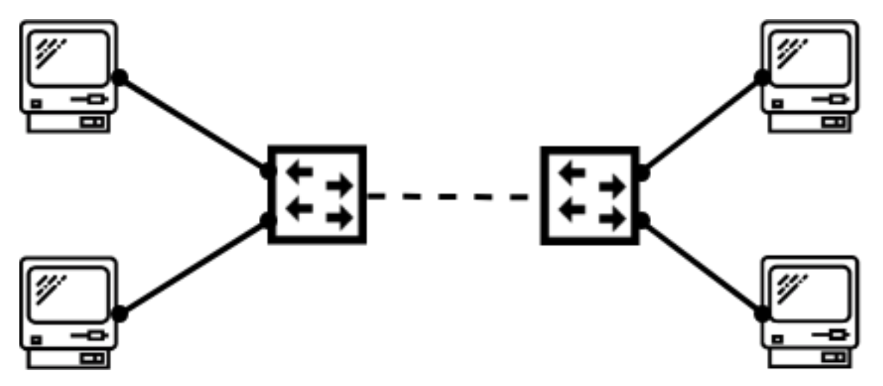
\includegraphics[scale=0.35]{mininet_topo.png}
\end{center}

Al correr el comando para levantar Mininet, se establece la IP del controlador que se va a utilizar. Esto es para que, luego, cuando corramos el controlador, el mismo pueda modificar los switches de la topología y maneje el control plane de la red de Mininet.

\subsection{POX - WIP}\label{pox}
Para implementar el controlador con OpenFlow, se utilizó la biblioteca POX. El controlador utiliza L2 learning para que los switches aprendan automáticamente a reenviar paquetes.

Para el firewall implementamos el metodo \texttt{\_handle\_ConnectionUp} que se encarga de instalar las reglas en el switch designado como firewall. Para esto, se lee el archivo \texttt{policies.json} que contiene las reglas a aplicar y se las traduce a objetos del tipo \texttt{ofp\_match}. Este objeto es un conjunto de criterios que se utilizan para identificar flujos de red en el contexto de utilizacion de OpenFlow. 

Luego entonces cuando un paquete llega al switch, se verifica si cumple con alguna de las reglas del firewall. En caso de cumplir con alguna regla, se descarta el paquete. En caso contrario, se lo deja pasar. 

\subsubsection{POX en ejecucion}

A continuación se observa lo que el controlador registra al iniciarse:
\begin{center}
 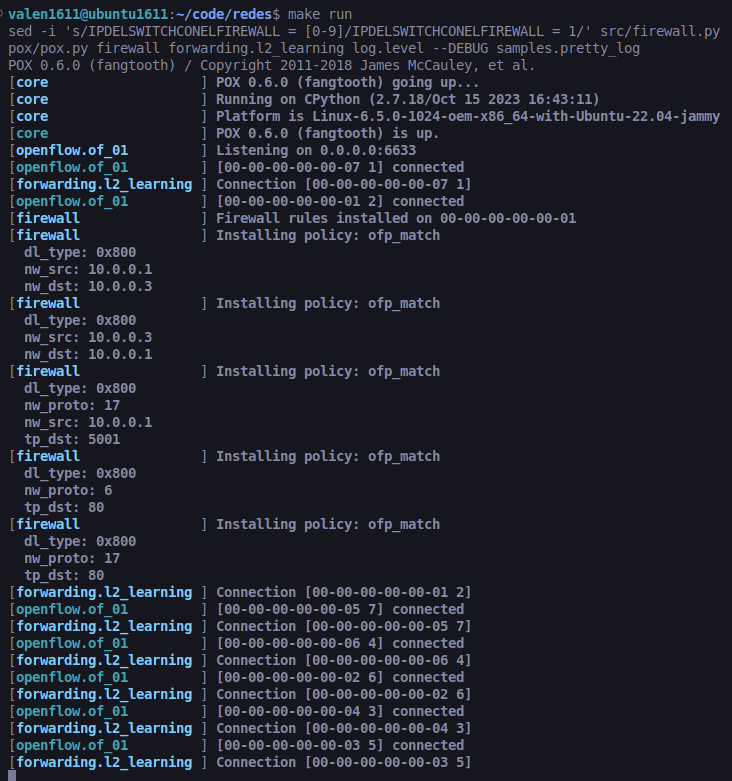
\includegraphics[scale=0.45]{pox_init.png}
 \captionof{figure}{Pox mostrando las reglas que instalo}
\end{center}


\subsection{Wireshark \& iperf}\label{wireshark-iperf} \


Para comprobar el correcto funcionamiento de la red y del Firewall, se utiliza iperf para simular clientes y servidores sin tener que configurarlos manualmente en los hosts de Mininet. 

Por otro lado utilizamos Wireshark para escuchar los paquetes que se envían en la red y verificar que el Firewall está funcionando correctamente.

A continuación se muestra el correcto funcionamiento del controlador, usando \texttt{pingall} dentro de Mininet y escuchando con Wireshark.

\begin{center}
  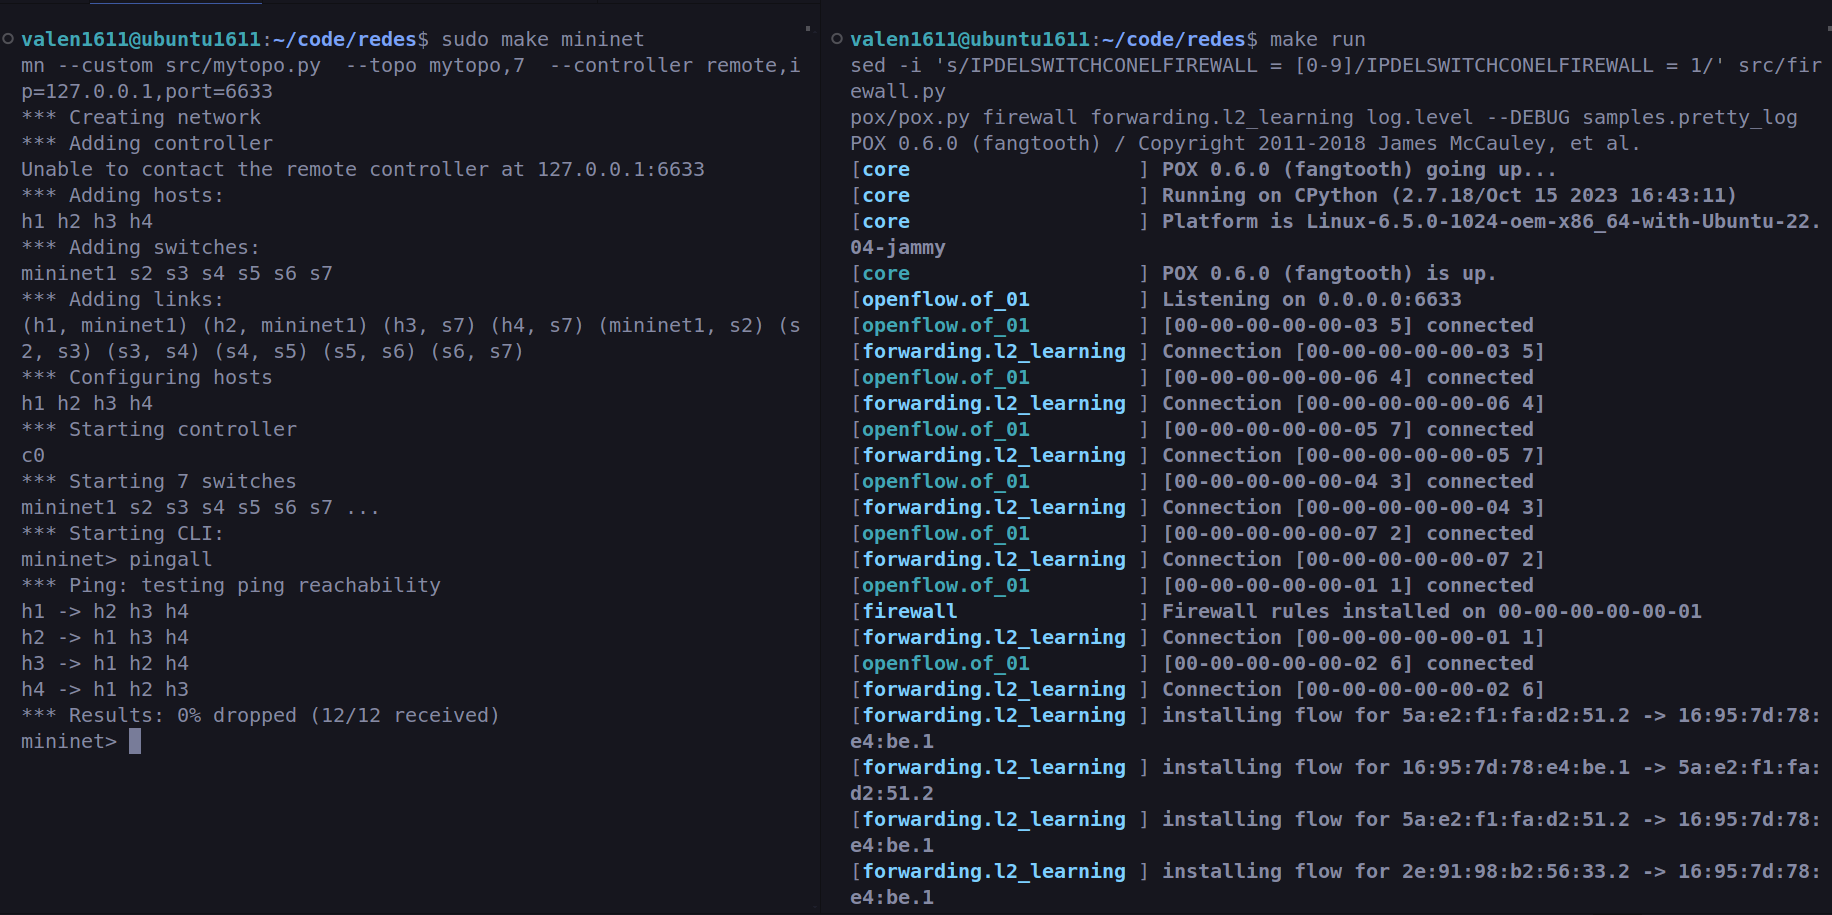
\includegraphics[scale=0.20]{mininet_pingall.png}
  \captionof{figure}{Mostrando pox con mininet a la vez}

\end{center}

\begin{center}
  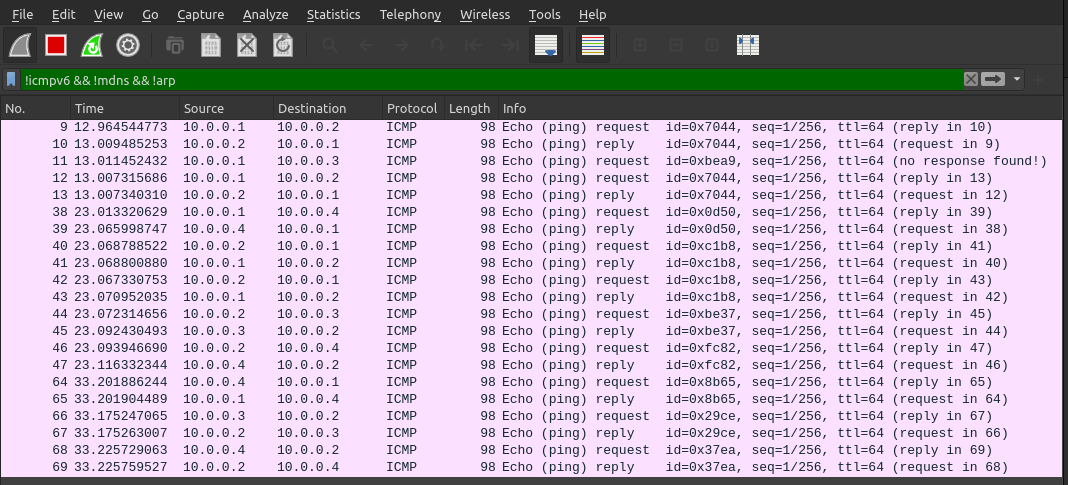
\includegraphics[scale=0.3]{pingAll_WS.png}
  \captionof{figure}{Wireshark con pingall}

\end{center}
  
Para comprobar que no solo funciona con ICMP, utilizamos iperf. Con iperf simulamos clientes y servidores, usando conexiones tanto TCP como UDP. En el ejemplo a continuación, el host h2 actúa como cliente y el host h3 actúa como servidor, comunicándose por TCP.

\begin{center}
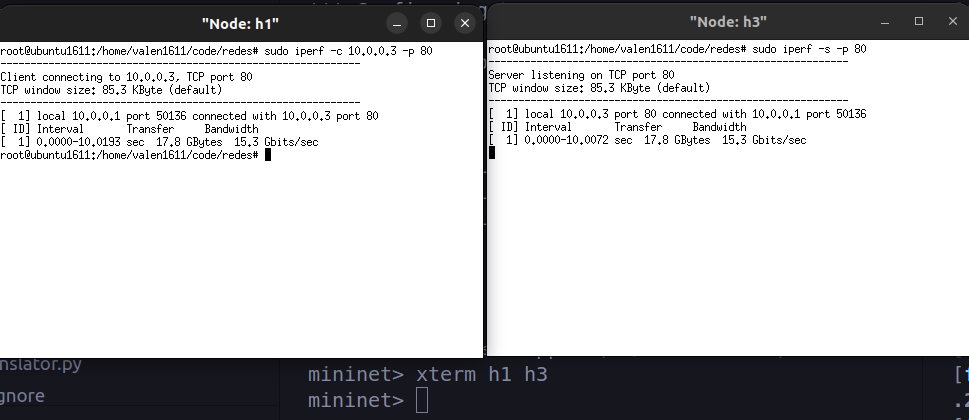
\includegraphics[scale=0.37]{mininet_iperf_basico.png}
\captionof{figure}{Hosts de Mininet con iperf basico}

\end{center}

\begin{center}
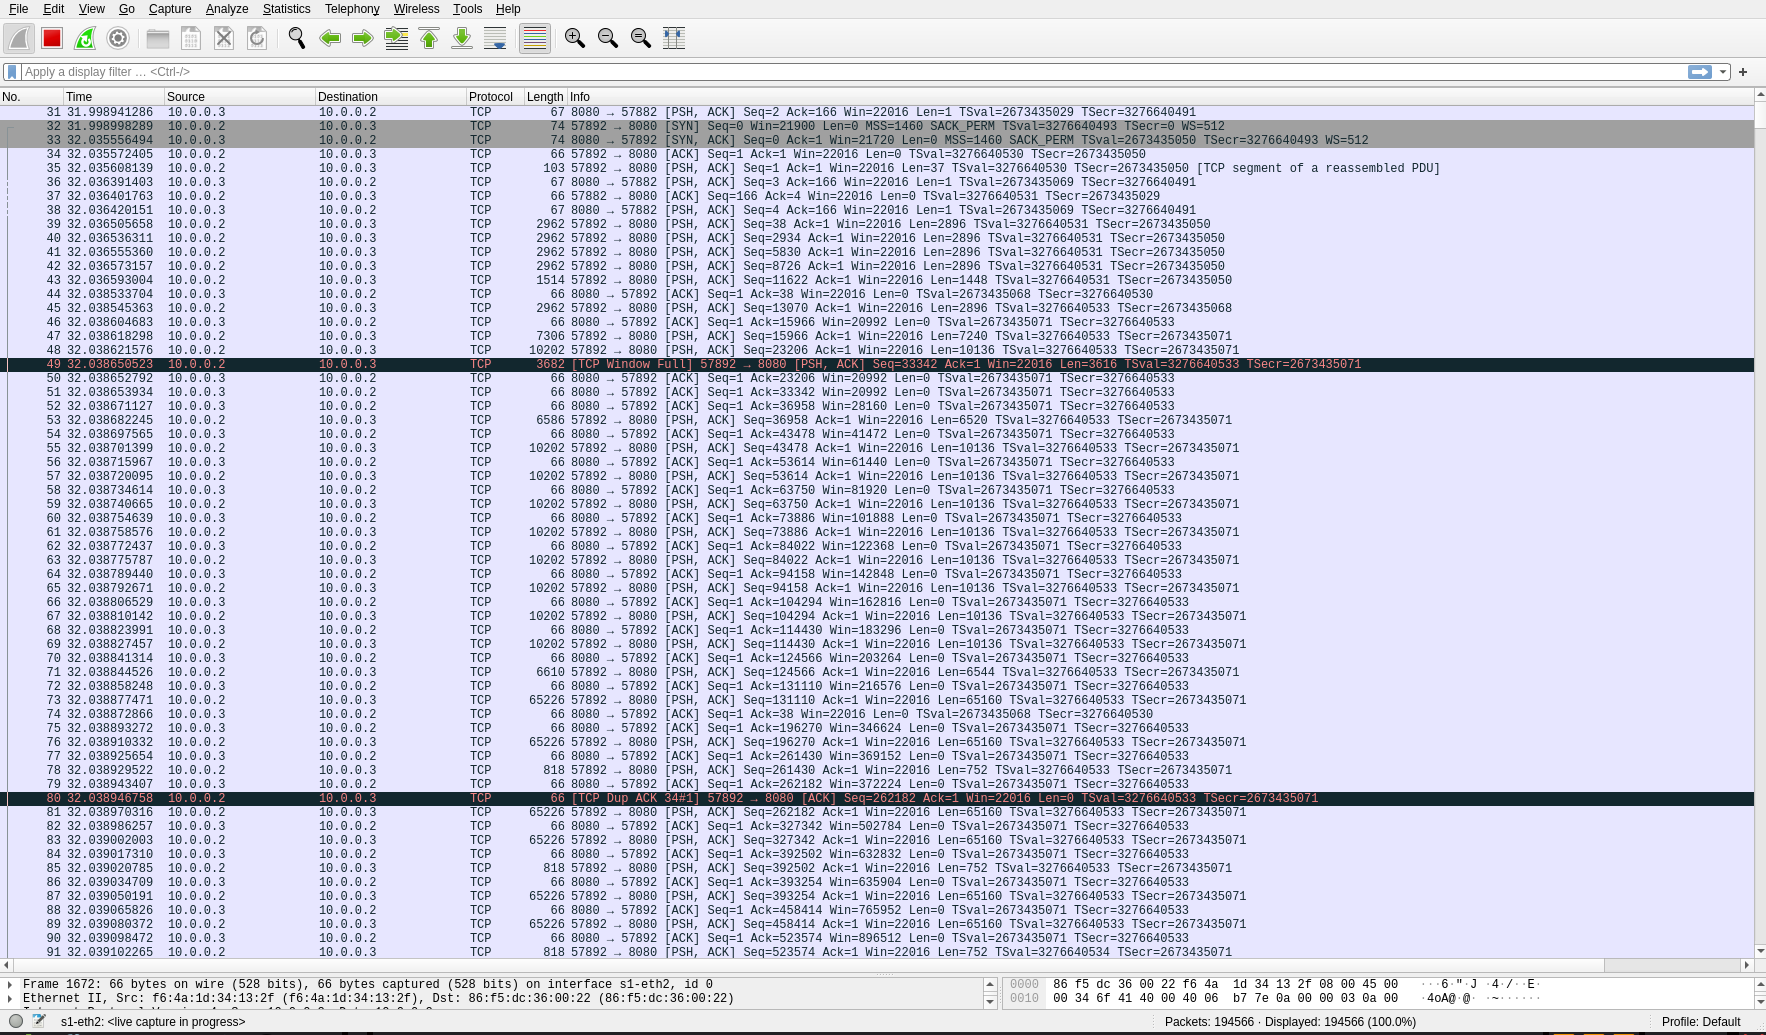
\includegraphics[scale=0.2]{iperfTCP.png}
\captionof{figure}{Imagen Traza Wireshark con el iperf basico}

\end{center}

\section{Resultados de simulaciones - WIP IMAGENES}\label{pruebas-wip}

\subsection{Puerto Destino 80}
Simulación para descartar todos los mensajes cuyo puerto destino sea 80. Se utilizan los hosts 1 y 4. 

\subsubsection{Reglas}
\begin{minted}{js}
{
    "policies":[
        {
            "dst_port": "80"
        }
    ]
}
\end{minted}

\subsection{Iperf}
\begin{center}
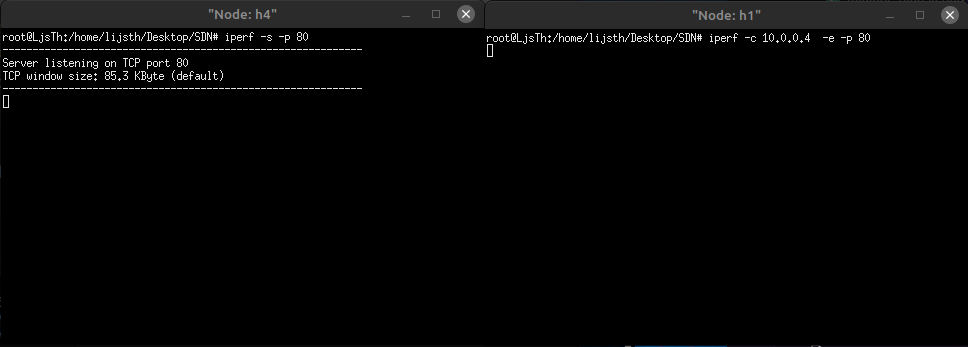
\includegraphics[scale=0.35]{iperf_port_80.png}
\captionof{figure}{Iperf cliente y servidor TCP que no se pueden comunicar por el puerto 80}
\end{center}

\subsubsection{Wireshark}
\begin{center}
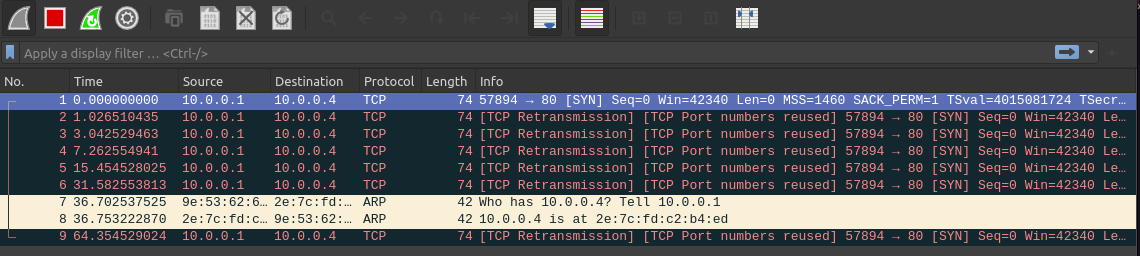
\includegraphics[scale=0.35]{bloq_80_port.png}
\captionof{figure}{Wireshark con puerto 80 bloqueado mostrando que no llega el SYN} 
\end{center}

\subsubsection{Logs del controlador}
\begin{center}
  \inputminted[fontsize=\footnotesize]{text}{informe/logs/Port_80_Log.txt}
\end{center}

\subsection{Host 1, Puerto 5001 y UDP}
Simulación para descartar todos los mensajes que provengan del host 1, tengan como puerto destino el 5001, y utilicen el protocolo UDP.
% WARNING: Poner todas las tildes. Como si fuesemos estudiantes de lingüistica (solo saben poner tildes)
\subsubsection{Reglas}
\begin{minted}{js}
{
    "policies":[
        {
            "src_ip": "10.0.0.1",
            "dst_port": 5001,
            "protocol": "UDP"
        }
    ]
}
\end{minted}



\subsection{Iperf}
\begin{center}
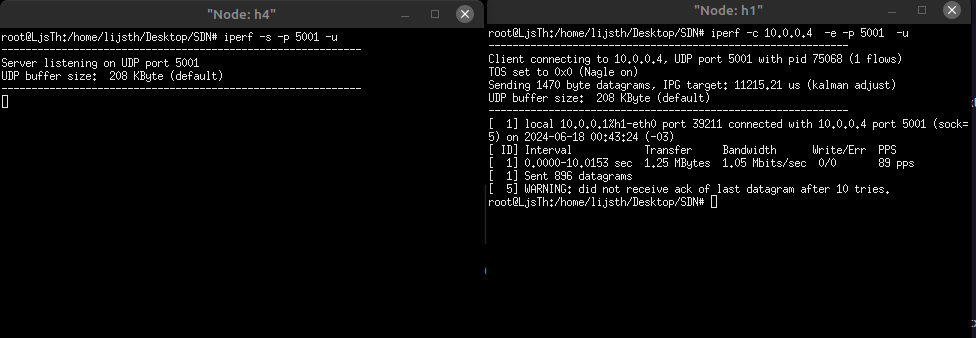
\includegraphics[scale=0.35]{Multi_Rules_UDP_P80_h1_Iperf.png}
\captionof{figure}{Iperf cliente en h1 y servidor en h4 UDP en puerto 5001 que no se pueden comunicar}
\end{center}

\subsubsection{Wireshark}
\begin{center}
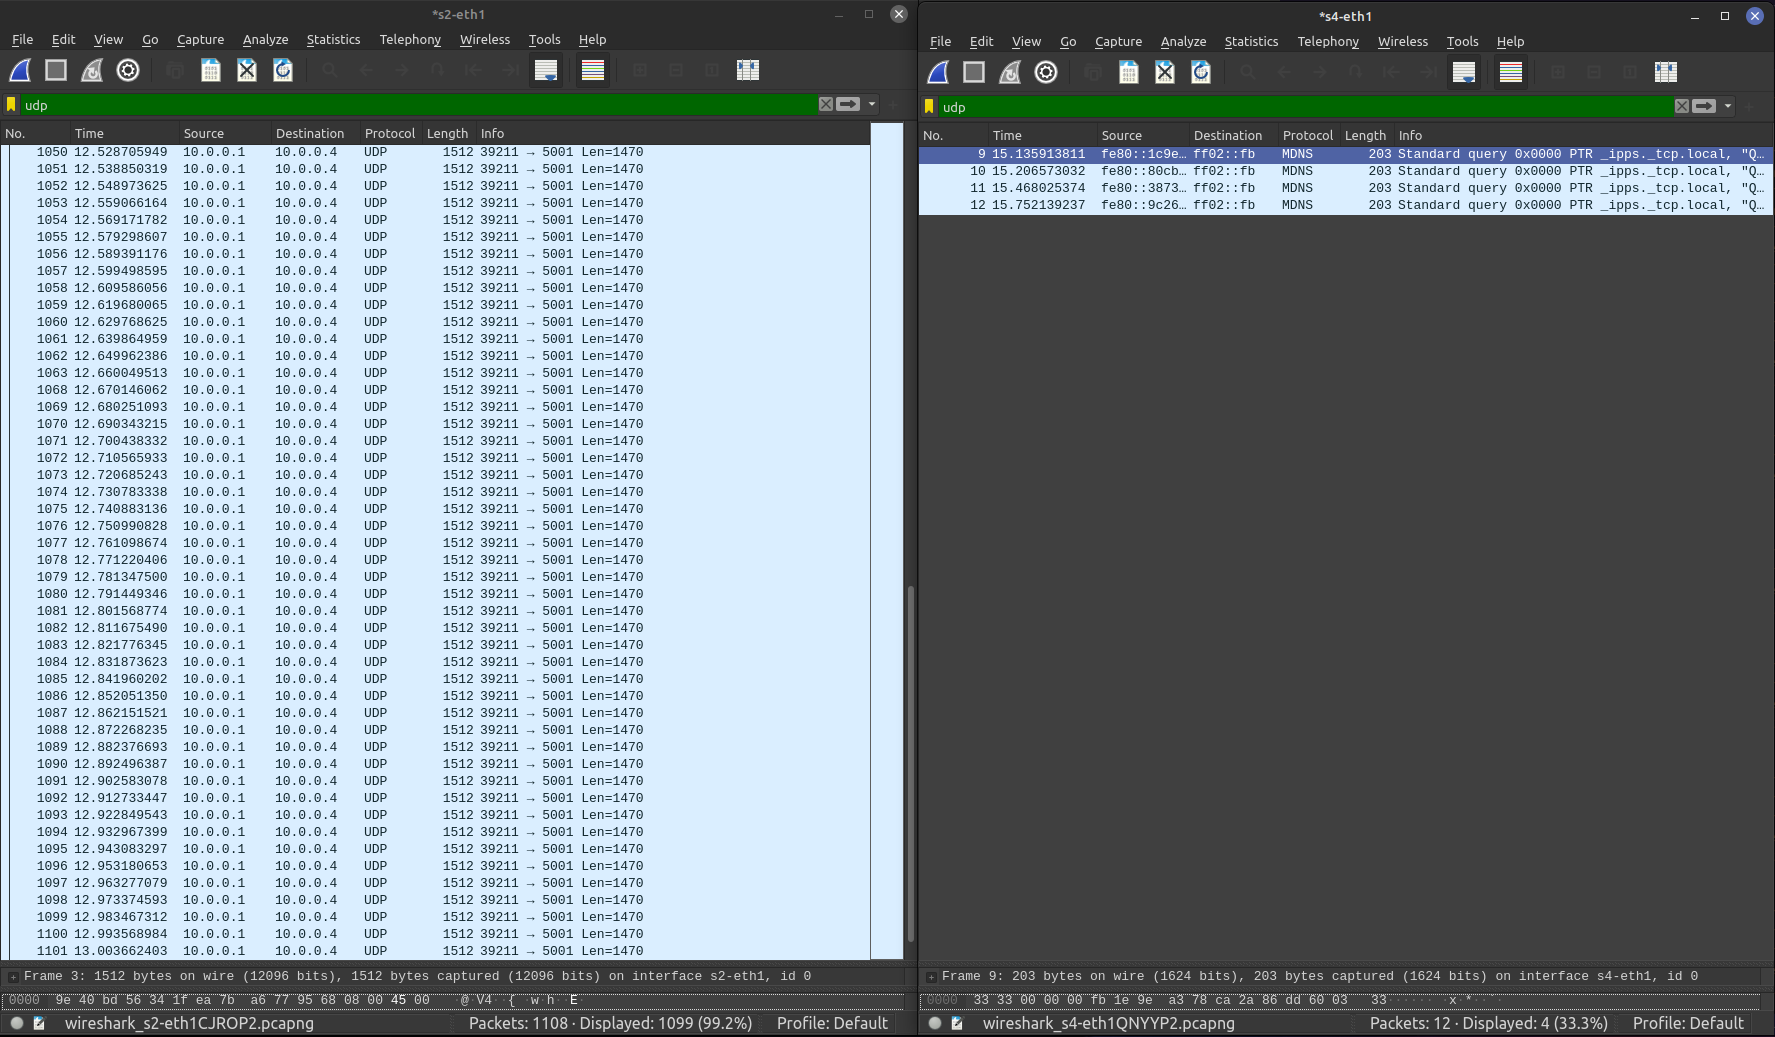
\includegraphics[scale=0.2]{Multi_Rules_WS_.png}
\end{center}

\subsubsection{Logs del controlador}
\begin{center}
  \inputminted[fontsize=\footnotesize]{text}{informe/logs/Multi_Rules_WS.txt}
\end{center}

\subsection{Dos hosts no se comunican entre sí}
Simulación donde se eligen dos hosts cualquiera, y los mismos no pueden comunicarse de ninguna forma. Utilizamos el comando pingAll de mininet para demostrar que no se pueden comunicar. Se utilizan los hosts 1 y 3.

\subsubsection{Reglas}
\begin{minted}{js}
{
    "policies":[
        {
            "banned_tuples": ["10.0.0.1", "10.0.0.3"]
        }
    ]
}
\end{minted}

\subsubsection{Wireshark}
\begin{center}
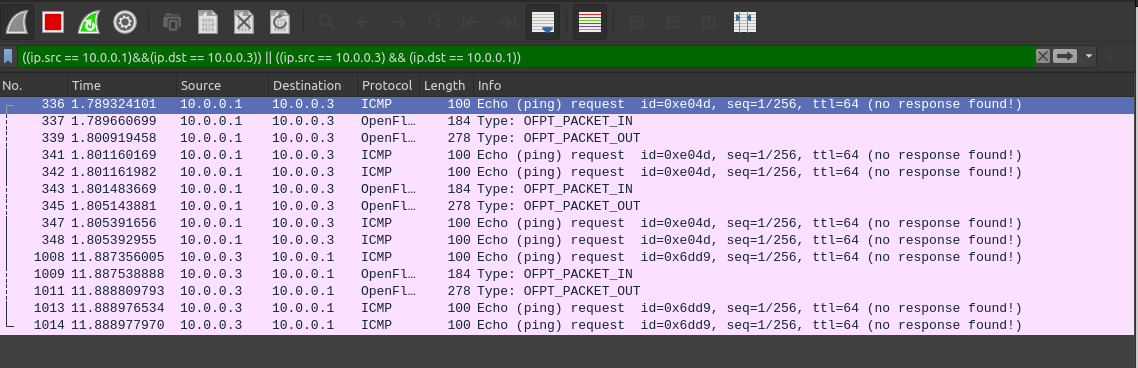
\includegraphics[scale=0.35]{Banned_Tuple_WS.png}
\captionof{figure}{Wireshark con Banned Tuple}
\end{center}


\subsubsection{Logs del controlador}
\begin{center}
  \inputminted[fontsize=\footnotesize]{text}{informe/logs/Banned_Tuple_Log.txt}
\end{center}


\subsection{Mininet PingAll}
\begin{center}
  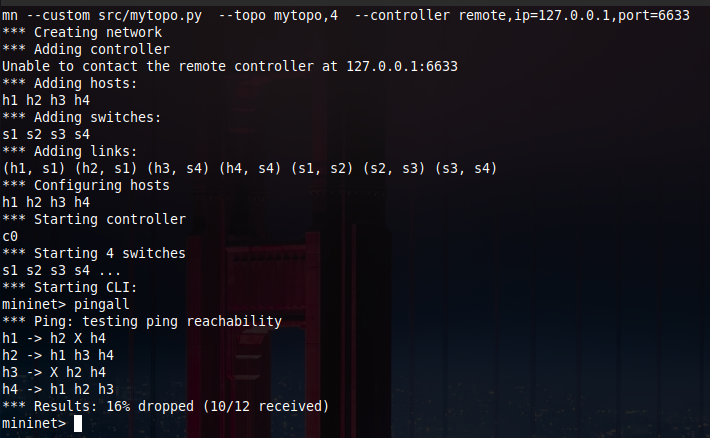
\includegraphics[scale=0.35]{Mininet_Banned_Tupled.png}
  \captionof{figure}{Mininet con Banned Tuple}
\end{center}

\section{Preguntas a responder}\label{preguntas-a-responder}

\subsection{¿Cuál es la diferencia entre un Switch y un router? ¿Qué tienen en común?}
Un switch y un router son dispositivos de red que permiten la comunicación entre múltiples dispositivos, pero operan en diferentes capas. Un switch trabaja en la capa 2 (enlace) y utiliza direcciones MAC para redirigir paquetes, facilitando la comunicación entre dispositivos dentro de una misma red local. Por otro lado, un router opera en la capa 3 (red) y utiliza direcciones IP para conectar múltiples redes simultáneamente, permitiendo la comunicación entre dispositivos en distintas redes. Ambos dispositivos toman los paquetes recibidos por sus puertos de entrada y los envían por los puertos de salida adecuados para alcanzar sus destinos finales.


\subsection{¿Cuál es la diferencia entre un Switch convencional y un Switch OpenFlow?}
La diferencia más importante entre un Switch convencional y uno OpenFlow es que el OpenFlow puede ser gestionado mediante software con un controlador centralizado, lo que permite automatizar y agilizar el proceso. Los switches convencionales no tienen el plano de control y el de datos desacoplados, por lo que configurarlos requiere más trabajo.


\subsection{¿Se pueden reemplazar todos los routers de la Internet por Switches OpenFlow? Piense en el escenario interASes para elaborar su respuesta.}
En principio, se podría integrar switches OpenFlow en una red, pero no es algo realmente factible debido a problemas de seguridad, rendimiento e interoperabilidad. En el contexto de interASes, manejar todo desde una única tecnología como OpenFlow podría facilitar la implementación de políticas de tráfico, pero crearía un single point of failure. Una vulnerabilidad en el protocolo OpenFlow expondría todo el Internet global. Además, sin routers, la implementación de NATs sería problemática. Los routers tradicionales, que implementan funciones en hardware, son más eficientes y rápidos, mientras que una red basada únicamente en switches OpenFlow estaría más congestionada. Además, los switches OpenFlow, como el POX, no implementan protocolos cruciales como BGP y OSPF, haciendo imposible la gestión completa de direcciones en una red global solo con switches OpenFlow.


\section{Conclusion}
Gracias a la tecnologia de Openflow; pudimos codificar un firewall dinamico. Este nos permitio describir un set de reglas para filtrar paquetes y luego instalar dichas reglas de forma remota a un switch.

\end{document}
